\documentclass[11pt]{article}

\newcommand{\cnum}{CS M146}
\newcommand{\ced}{Winter 2019}
\newcommand{\ctitle}[3]{\title{\vspace{-0.5in}\cnum, \ced\\Problem Set #1: #2\\Due #3}}
\usepackage{enumitem}
\newcommand{\solution}[1]{{{\color{blue}{\bf Solution:} {#1}}}}
\usepackage[usenames,dvipsnames,svgnames,table,hyperref]{xcolor}
\usepackage{graphicx}
\usepackage[tbtags]{amsmath}
\usepackage[hang, small,labelfont=bf,up]{caption} % Custom captions under/above floats in tables or figures
\usepackage{booktabs} % Horizontal rules in tables


\renewcommand*{\theenumi}{\alph{enumi}}
\renewcommand*\labelenumi{(\theenumi)}
\renewcommand*{\theenumii}{\roman{enumii}}
\renewcommand*\labelenumii{\theenumii.}


\begin{document}
\ctitle{1}{Decision Trees}{Jan 28, 2019}
\author{Tian Ye}
\maketitle

\newpage

\section{Maximum Likelihood Estimation}
\begin{enumerate}
\item 

\solution{
The likelihood estimation is given by the following:
\begin{align}
L(\theta) &= \prod_{i=1}^{n} P_{\theta}(X_{i}) \\
	     &= \prod_{i=1}^{n} \theta^{X_{i}}(1-\theta)^{1-X_{i}} \\
	     &= \theta^{x_{1}}(1-\theta)^{x_{0}}
\end{align}
Where $x_{1}$ counts the number of cases which $X_{i} = 1$ and  $x_{0}$ counts the number of cases which $X_{i} = 0$. \\
The order of the individual random variables $X_{i}$ do not matter as they are independent from one another.
}

\vspace{1cm}

\item
\solution{
Taking the log likelihood of the previous expression:
\begin{align}
\ell(\theta) &= \log(\theta^{x_{1}}(1-\theta)^{x_{0}}) \\
                  &= x_{1}\log(\theta) + x_{0}\log(1-\theta)
\end{align}

Taking the first and second derivatives of $\ell(\theta)$ with respect to $\theta$:
\begin{align}
\ell^{\prime}(\theta) &= \frac{x_{1}}{\theta} - \frac{x_{0}}{1-\theta}\\
\ell^{\prime\prime}(\theta) &= -\frac{x_{1}}{\theta^2} - \frac{x_{0}}{(1-\theta)^2}\\
\end{align}

Since $\ell^{\prime\prime}(\theta) < 0$, the function is always concave down. \\
We can therefore set $\ell^{\prime}(\theta) = 0$ to solve for the MLE:
\begin{align}
\theta_{MLE} = \frac{x_1}{x_{1}+x_0}
\end{align}
}
\newpage


\item
\solution{
\begin{figure}[!htbp]
    \centering
    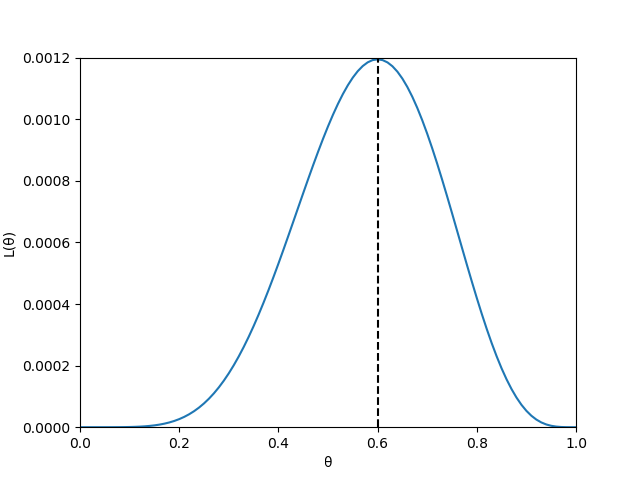
\includegraphics[width=3in]{1c.png}
    \caption{The figure above does agree with Equation 9 given in the previous section; we can see this as the maximum is at $\theta = 0.6$, which corresponds with $\frac{6}{4 + 6}$.}
\end{figure}
}

\item
\solution{
\begin{figure}[!htbp]
    \centering
    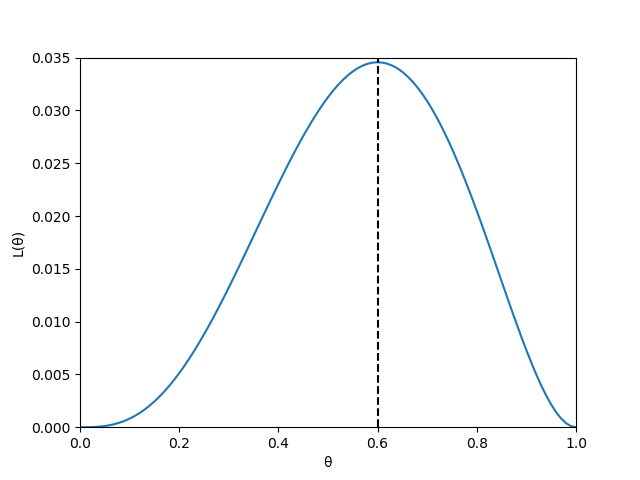
\includegraphics[width=3in]{1di.png}
    \caption{By decreasing the number of data points while maintaining the ratio of 1s to 0s, the likelihood plot keeps the same MLE while having a wider spread and a lower likelihood. This is because we have less data; therefore we are less confident.}
\end{figure}
\newpage

\begin{figure}[!htbp]
    \centering
    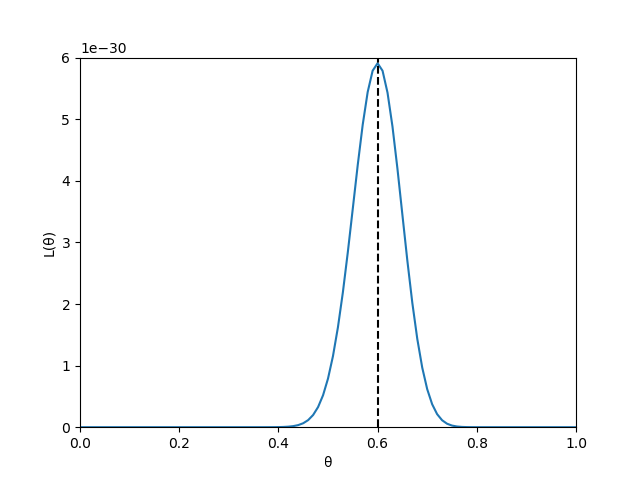
\includegraphics[width=3in]{1dii.png}
    \caption{By increasing the number of data points while maintaining the ratio of 1s to 0s, the likelihood plot keeps the same MLE while having a narrower spread and a higher likelihood. This is because we have more data; therefore we are more confident.}
\end{figure}

\begin{figure}[!htbp]
    \centering
    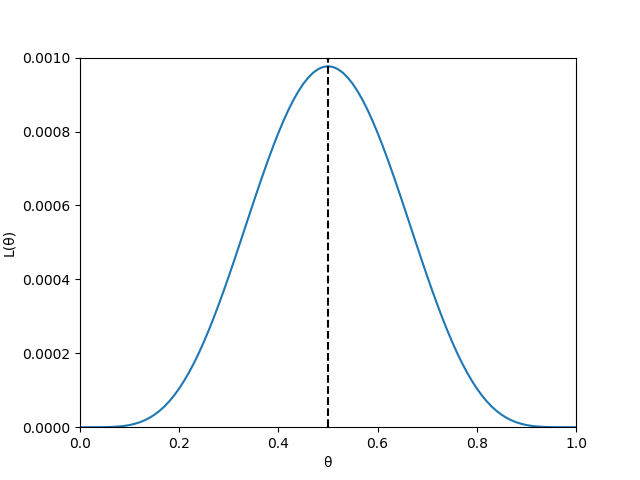
\includegraphics[width=3in]{1diii.png}
    \caption{By maintaining the same number of data points while changing the ratio of 1s to 0s, the likelihood plot shifts the MLE while maintaining the spread and likelihood. Intuitively, this is because we have the same number of data points.}
\end{figure}
}
\end{enumerate}
\newpage

\section{Splitting Heuristic for Decision Trees}
\begin{enumerate}
\item
\solution{The best 1-leaf decision tree makes an error $\frac{1}{8}$ of the time.  The decision tree is as follows: $Y = 0$ if and only if $X_1 = X_2 = X_3 = 0$. \\
This leaves us with $2^{n-3}$ remaining binary vectors; hence the error is $\frac{2^{n-3}}{2^n} = \frac{1}{8}$.
}
\vspace{1cm}

\item
\solution{There does not exist a split that reduces the number of mistakes. If we split on $X_1$, $X_2$, or $X_3$, it will create a tree in which one leaf only contains 1s and the other leaf contains 1s with a proportion of $\frac{3}{4}$. Splitting on a value of $n \geq 4$ will create two leaves where the proportion of 1s is $\frac{7}{8}$. In both cases the tree will always predict 1, leaving an error rate of $\frac{1}{8}$.
}
\vspace{1cm}

\item
\solution{$\frac{1}{8}\log(8) + \frac{7}{8}\log(\frac{8}{5})$ = 0.543
}
\vspace{1cm}

\item
\solution{By splitting on $X_1$, $X_2$, or $X_3$, we can reduce the entropy on the output $Y$. The new entropy following the split is as follows: \\
$\frac{1}{2}[\frac{1}{4}\log(4)+\frac{3}{4}\log(\frac{4}{3})]= 0.406$ \\
This reduces the entropy on $Y$ by 0.137.
}
\newpage
\end{enumerate}

\section{Entropy and Information}
\begin{enumerate}
\item
\solution{We know that the entropy must fall within the range of $0 \leq H(S) \leq 1$ using the following:
\begin{align}
B(q) &= -q\log(q) - (1-q)\log(1-q)
\end{align}
For a set containing $p$ positive examples and $n$ negative examples, $H(S) = B(\frac{p}{n+p})$. We will show that $0 \leq H(S)$ by setting $p=0$ and $n$ to some value greater than 0:
\begin{align}
B(\tfrac{0}{n+0}) &= -q\log(q) - (1-q)\log(1-q) \\
B(0) &= 0\log(0) - (1-0)\log(1-0) \\
H(S) &= 0
\end{align}
For any value of $p$ such that $0 \leq p \leq n$, $H(S)$ increases and approaches 1 as $q$ increases towards $\frac{1}{2}$. We know this from the first and second derivatives of $B(q)$:
\begin{align}
B(q)^{\prime} &= \log(1-q) - \log(q) \\
B(q)^{\prime\prime} &= -\frac{1}{q} - \frac{1}{1-q}
\end{align}
Since $q$ is given by $(\tfrac{p}{n+p})$, $q$ is bound between 0 and 1. Furthermore, we know that the function maximizes at $q = \frac{1}{2}$ as the first derivative at that value is 0 and the second derivative is strictly negative for the interval $ 0 \leq q \leq 1$. Once $p = n$, we yield the following: 
\begin{align}
B(\tfrac{n}{2n}) &= -q\log(q) - (1-q)\log(1-q) \\
B(\tfrac{1}{2}) &= -\tfrac{1}{2}\log(\tfrac{1}{2}) - (1-\tfrac{1}{2})\log(1-\tfrac{1}{2}) \\
H(S) &= 1
\end{align}
As $p$ increases past $n$, the value $q$ once again begins to decrease towards 0, and as such, $H(S)$ decreases back towards 0. Hence, $0 \leq H(S) \leq 1$.
}
\newpage

\item
\solution{
Given that $S_1, S_2, S_3,...,S_k$ are disjoint subsets of $X_j$ and that the ratio $\tfrac{p_k}{p_{k}+n_k}$ is the same for all $k$, we can state the following:
\begin{align}
H(S_k) &= B(\tfrac{p_k}{p_k+n_k}) \\
H(S | X_j) &= H(S_1)\tfrac{p_1+n_1}{p+n} + ... + H(S_k)\tfrac{p_k+n_k}{p+n} \\
H(S | X_j) &= H(S)\tfrac{p_1+n_1+p_2+n_2+...+p_k+n_k}{p+n} \\
H(S | X_j) &= H(S)\tfrac{p+n}{p+n} \\
H(S | X_j) &= H(S) \\
H(S | X_j) &= B(\tfrac{p}{n+p})
\end{align}
Therefore we can see that splitting the set S by the attribute $X_j$ gains 0 information:
\begin{align}
H(S | X_j) - H(S)= B(\tfrac{p}{n+p}) - B(\tfrac{p_k}{p_k+n_k}) = 0
\end{align}
}
\end{enumerate}
\newpage


\section{k-Nearest Neighbor}
\begin{enumerate}
\item
\solution{Setting a value of $k=0$ minimizes the training set error, achieving a set error of 0. This is because the closest training set data point to a given point is itself, causing it to achieve perfect accuracy. This training set is not a reasonable estimate of test set error, as this value of $k$ essentially causes the algorithm to ``memorize'' the training set. \\
Achieving an error of 0 is impossible if the test set is distinct from the training set, as the program would not have ``learned'' anything from the test set due to overfitting. \\
Consequently, given a distinct testing set from the training set, the error would be very high with a value of $k=0$.
}
\vspace{1cm}

\item
\solution{ $k=5$ minimizes the LOOCV error as it guarantees that the two groups of five circles and five astericks will be correctly classified. As a result, only the two groupings of two circles and two astericks will fail. \\
This leads to an error rate of $\tfrac{2}{7}$. Setting $k=5$ is a better measure of test set performance as it is nonzero and therefore realistic.
}
\vspace{1cm}

\item
\solution{The LOOCV error for $k=1$ is $\frac{5}{7}$, while the LOOCV error for $k=14$ is 1. \\
The disadvantage of using a large $k$ is that the predicted value for a given data point depends on the remaining data points; for example, in this instance, setting $k=14$ will cause an error rate of 100\% as there will be 6 remaining data points of the selected point and 7 remaining data points for the other selected point.\\
 The disadvantage of using too small a data point is that the classification of a given point will be based solely on the nearest data value. This will cause issues in patterns such as a checkerboard, where related points lie along diagonals but the closest and unrelated points lie along the rows and columns; consequently, this will cause high amounts of error.
}
\end{enumerate}
\newpage

\section{Programming Exercises: Applying Decision Trees}
\begin{enumerate}
\item
\solution{
\begin{figure}[!htbp]
    \centering
    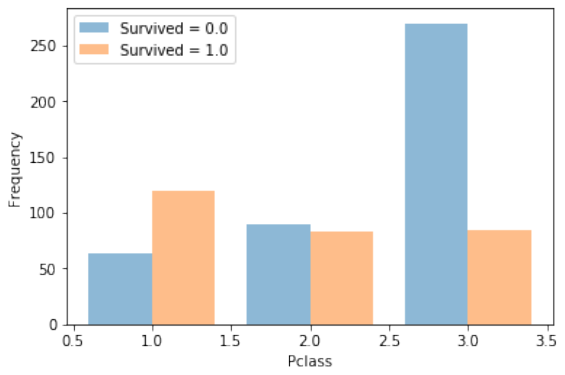
\includegraphics[width=3in]{5a-ticket.png}
    \caption{We can note that for ticket class 1, the number of survivors was approximately double that of those that did not survive. For ticket class 2, the number of survivors compared to fatalities was approximately the same. For ticket class 3, the number that did not survive was nearly three times that did survive. Thus it can be concluded that the wealthier the passenger, the higher the likelihood of survival.}
\end{figure}
\begin{figure}[!htbp]
    \centering
    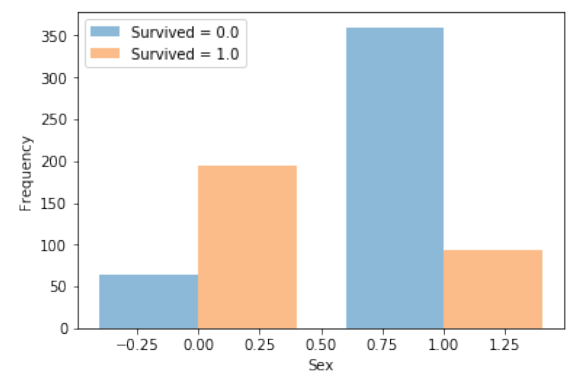
\includegraphics[width=3in]{5a-sex.png}
    \caption{We can note that for males, the survival rate was significantly lower than that of females. Namely, approximately 200 females survived while 50 did not, while for males 350 did not survive while only about 100 did.}
\end{figure}
\begin{figure}[!htbp]
    \centering
    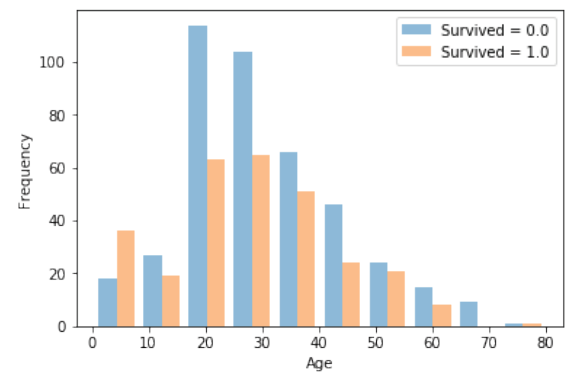
\includegraphics[width=3in]{5a-age.png}
    \caption{We can note that with the exception of the youngest age group, those younger than 10 years old, more passengers perished than those that survived. The data set as a whole is right skewed, and the highest fatality rates were generally found for those in the age range of 20 - 40 years old.}
\end{figure}
\begin{figure}[!htbp]
    \centering
    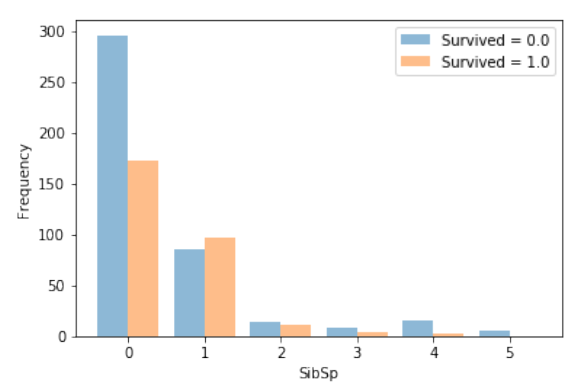
\includegraphics[width=3in]{5a-sibsp.png}
    \caption{We can note that the data as a whole is heavily skewed right, with those having 1 other sibling or spouse having a higher survival rate than the other categories. The other sibling-spouse categories had the similar surivival rates as the 0 group, albeit with much lower frequencies.}
\end{figure}
\begin{figure}[!htbp]
    \centering
    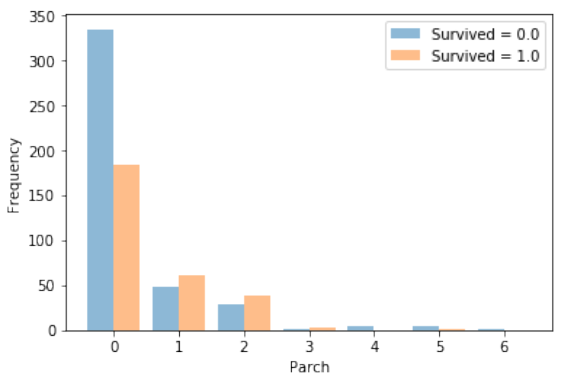
\includegraphics[width=3in]{5a-parch.png}
    \caption{We can note that the data as a whole is heavily skewed right, with those having 1 or 2 other parents or children having a higher survival rate than those with none. Those with none suffered approximately a 66\% mortality rate, whereas those with 1 or 2 had more surviving than perishing. The other parent-children categories have nearly negligible frequencies.}
\end{figure}
\begin{figure}[!htbp]
    \centering
    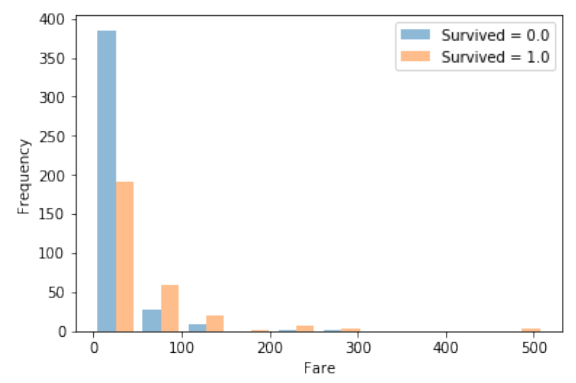
\includegraphics[width=3in]{5a-fare.png}
    \caption{We can note that the data as a whole is heavily skewed right, and that those that payed less than \$100 as a whole had a much lower survival rate than those who did not. Notably, those in the \$50 category suffered a 66\% mortality rate while those above suffered a 33\% mortality rate.}
\end{figure}
\begin{figure}[!htbp]
    \centering
    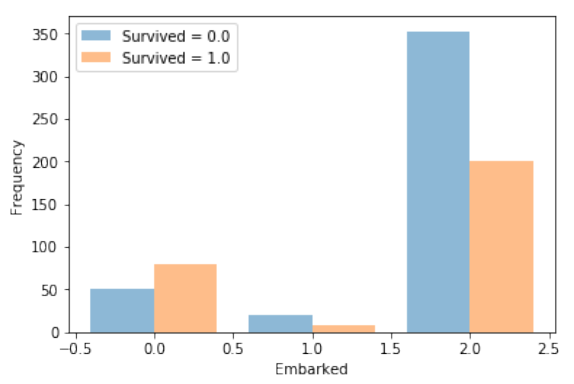
\includegraphics[width=3in]{5a-embarked.png}
    \caption{In this graph, the three x-axis values are Cherbourg, Queenstown, and Southampton. Passengers from Cherbourg enjoyed the highest survival rate, while those from Queenstown and Southampton had more fatalities than survivals. However, the number of survivals from Southampton was higher than that of Cherbourg, owing to the much higher number of passengers departing from Southampton.}
\end{figure}
}
\vspace{1cm}

\item
\solution{After implementing RandomClassifier, I achieved the training error value of 0.485.
}
\vspace{1cm}


\item
\solution{Using the entropy criterion for information gain, the training error of the DecisionTreeClassifier is 0.014.
}
\vspace{1cm}

\item
\solution{
\begin{table}[!htbp]
\caption{Investigating Various Classifiers}
\centering
\scalebox{1}{
\begin{tabular}{lcc}
\toprule
\cmidrule{1-3}
Model Type & train\_err & test\_err \\
\midrule
Majority & 0.404 & 0.407 \\
Random & 0.489 & 0.487 \\
Decision Tree & 0.012 & 0.241 \\
\bottomrule
\end{tabular}}
\end{table}
}
\newpage

\item
\solution{
\begin{figure}[!htbp]
    \centering
    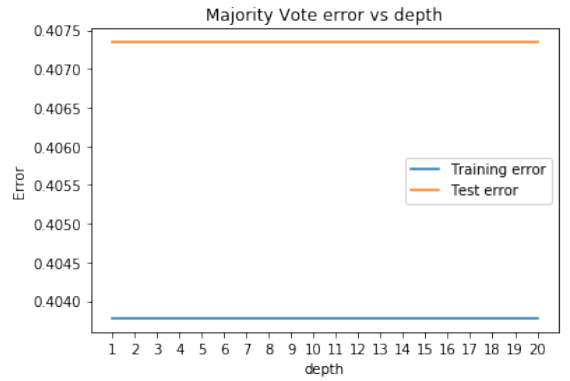
\includegraphics[width=3in]{5e-majority.png}
    \caption{We can tell by the figure above that the Majority Vote Classifier does not depend on depth; therefore there is no overfitting and no best value for depth.}
\end{figure}
\vspace{1cm}

\begin{figure}[!htbp]
    \centering
    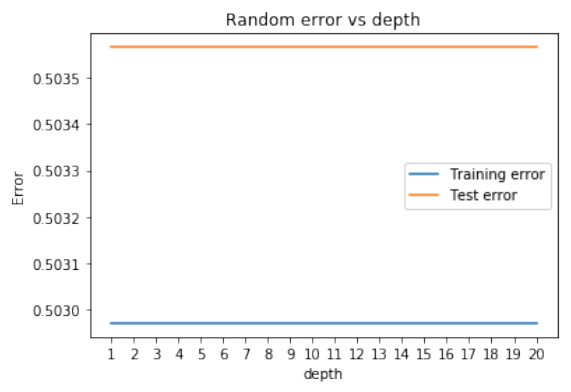
\includegraphics[width=3in]{5e-random.png}
    \caption{We can tell by the figure above that the Random Classifier does not depend on depth; therefore there is no overfitting and no best value for depth.}
\end{figure}
\vspace{2cm}

\begin{figure}[!htbp]
    \centering
    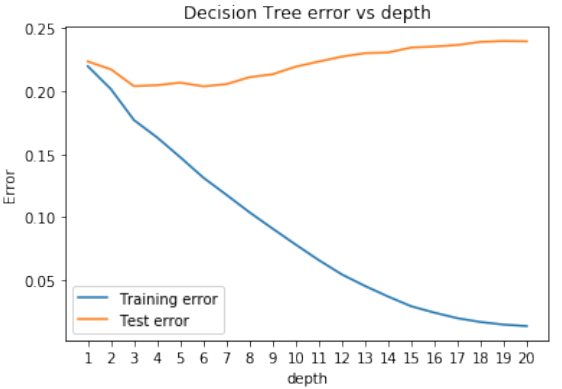
\includegraphics[width=3in]{5e-tree.png}
    \caption{Viewing the figure above, we can see clear signs of overfitting: as the depth increases, the training error steadily decreases while the test error first decreases before increasing again. This shows that as the decision tree becomes more complex as the depth increases, it becomes less adapatable and is unable to generalize new data and examples in the testing set, leading to higher error rates. The ideal depth for the Decision Tree Classifier is 6. At this value, the error is minimized at a value of 0.203776223776.}
\end{figure}
\vspace{1cm}
}

\item
\solution{
\begin{figure}[!htbp]
    \centering
    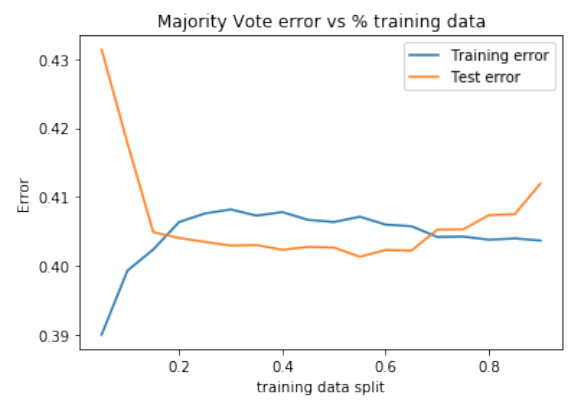
\includegraphics[width=3in]{5f-majority.png}
    \caption{Viewing the figure above, we can see that until 20\%, each increase in the training data split leads to a lower test\_err and a higher train\_err until they center around 40\% error for both. Afterwards, they remain relatively constant. This is because as the training set increases in size, it becomes more representative of the actual data, leading to higher accuracy in relation to the test error.}
\end{figure}
\vspace{1cm}
\begin{figure}[!htbp]
    \centering
    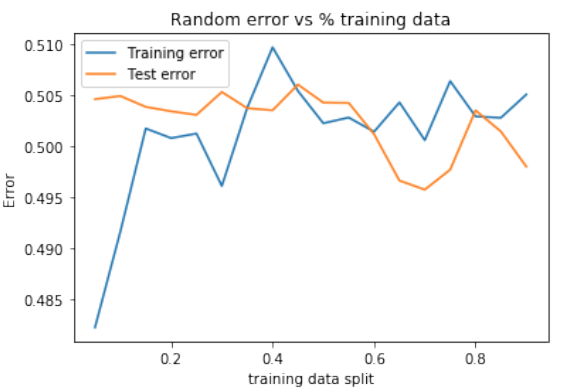
\includegraphics[width=3in]{5f-random.png}
    \caption{Viewing the figure above, we can see that as the training set increases up to 20\% error, the training error increases steadily until it reaches around 50\%. As the training set increases up to 95\%, both the training error and the test error fluctuate between 50\% and 51\%. This can be attributed to the fact that Random Classifier will classify at random examples based on a percentage of the entire training set: the random nature of the data assignment to classes will keep random error fluctuating across a center error value.}
\end{figure}
\begin{figure}[!htbp]
    \centering
    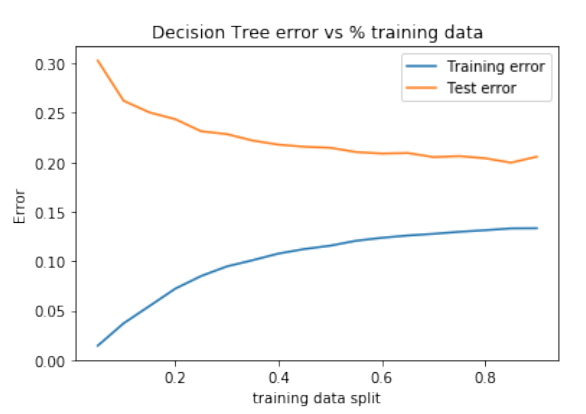
\includegraphics[width=3in]{5f-tree.png}
    \caption{Viewing the figure above we can see that as the training set increases, the training error decreases while the test error decreases, with nearly 10\% change for both test and training error. This is attributed to the fact that as the training set increases, the decision tree will increase in depth. This creates more options for the training set examples to be matched with, increasing error. At the same time, the tree improves at generalizing, decreasing test error.}
\end{figure}
\vspace{1cm}
}
\end{enumerate}
\end{document}